\chapter{Adiabatic process on gate model}

Adiabatic computation


In practical implementation, adiabatic model of quantum computation
has many advantages in scale, speed and formulation of problem to run on the system.
On the gate model, we consider many approximation formula and representation of the evolution operator. 
The reason was that we cannot know exactly what form of the time-evolution operator form corresponding to the given hamiltonian matrix;hermite. 
However, in adiabatic computation, the unitary transformation is a \textbf{job of nature}. 
Only things we have to consider are how to apply the Hamiltonian to the given qubit system and 
accelerating convergence speed enough to use in calculation.
This computation model has very huge benefit in binary optimization problem than the gate model computation.

In this chapter, we are going to simulate adiabatic
process on gate model computer and compare the result obtained
from a commercial adiabatic process machine.

\section{Formulation for Adiabatic computing}

Adiabatic theorem states that if the system hamiltonian is varying slowly, 
the final state of the system is remained in eigenstate of finial hamiltonian 
which is corresponding eigenstate of the initial hamiltonian eigenstate.

The term slowly is very important, it depends on the initial and final hamiltonian of the system. 
If the evolution time is $T$, and the eigenvalues of initial and final hamiltonian are $E_i$
and, $E_f$, the evolution time must satisfy next,

\begin{equation}
    \frac{2 \pi}{|E_f - E_i| << T}
\end{equation}

That is to solve the system with adiabatic method, we have to manipulate the time, $T$.
It is called by \textit{adiabatic configuration}. 
The configuration depends on the initial and final system, 
so the determination requires some physical intuition by the researcher.

\begin{equation}
    \mathcal{H}_{adia} (f(s), T) = T(1- f(s)) \mathcal{H}_{initial} + f(s) \mathcal{H}_{solve}
\end{equation}

Our major concern is a ground state of $\mathcal{H}_{solve}$.
We can expect the system to be a ground state through adiabatic process,
if the initial system state was a ground state of $\mathcal{H}_{inital}$.
That is, with adiabatic process, we can obtain the target system ground state 
using well-known system.
The requirement is an appropriate Hamiltonian, $\mathcal{H}_{initial}$.
It must have well-known ground state and 
their implementation should practically be efficient.
Common Hamiltonian is a $\mathcal{H}_{inital} = - \sum_{i} \sigma_{X, i}$.
Its ground state is a $|+\rangle^{\otimes n}$.

\begin{center}
    \begin{quantikz}
        \lstick{$| 0_{0} \rangle$} &\gate{H}& \rstick{$| + \rangle$}  \\
        \lstick{$| 0_{1} \rangle$} &\gate{H}& \rstick{$| + \rangle$} \\
        \wave&& \\
        \lstick{$| 0_{n} \rangle$} &\gate{H}& \rstick{$| + \rangle$}
    \end{quantikz} = $|+\rangle^{\otimes n}$
\end{center}

The common annealing solutions, such as D-Wave and QuEra, also apply the adiabatic theorem to their initialization process and Hamiltonian form. 
Quantum annealing is fundamentally based on the phenomenon of quantum fluctuation; 
however, the starting and final stages, as well as the evolving process, follow the adiabatic theorem. 
That is why they offer some annealing time and initial state parameters to the user API. 
Some problems require much more time to achieve the appropriate adiabatic process

\section{Naive Implementation}

The previous simulations were time-independent
Hamiltonian systems, but adiabatic process is 
using a time-dependent Hamiltonian.
The commutation problem still arises in here.
If the $H(t_1)$ and $H(t_2)$ are not commuting, 
then we cannot apply the usual exponential formula.

Still, product formula work well except the additional error 
term was added to the system.

We can approximate this process with generating step Hamiltonians as 

\begin{equation}
    H_qc(t) = \left( 1- \frac{t}{T}\right) \mu H_i + \left( \frac{t}{T}\right) H_{solve}
\end{equation}

where, $\mu$ is a wieght coefficient of initial state.

%\begin{algorithm}
%    \caption{Adiabatic Process Approximation}\label{alg:naive_adiabatic}
%    \begin{algorithmic}
%    \Require $H_i, \mu, H_f$ \Comment{Initial Hamiltonian}
%    \Ensure $y = x^n$
%    \State $y \gets 1$
%    \State $X \gets x$
%    \State $N \gets n$
%    \While{$i < step$}
%    \If{$N$ is even}
%        \State $X \gets X \times X$
%        \State $N \gets \frac{N}{2}$  \Comment{This is a comment}
%    \ElsIf{$N$ is odd}
%        \State $y \gets y \times X$
%        \State $N \gets N - 1$
%    \EndIf
%    \EndWhile
%    \end{algorithmic}
%    \end{algorithm}

\begin{lstlisting}
    [Adiabatic Processs Approximation]

    H_i <- initial hamiltonian
    mu <- weight of the H_i
    H_f <- problem hamiltonian
    --------------------------------------------------
    func_evolve(t, H, tn): 
        Applying time evolution operator on state
            evolution time: t, 
            hamiltonian: H 
            trroter decompose level: tn.
    
    func_Hqc(s, t, mu): (1-s/t) mu * H_i + (s/t) H_f
        Return instaneous hamiltonian of the given time step: s.
        --------------------------------------------------
    [Defined Adabatic schedule parameters]
    
    T <-  # total evolution time
    steps <-  # time difference step number
    dt <- T/steps
    
    trotter_num <- # trotter decompose level
    
    [Prepare the circuit]
    
    initiate the system with Hadamard basis |+>
    
    while i < step
        t = dt*i
        H_t = func_Hqc(t, T, mu)
        ----------------
        func_evolve(dt, H_t, trotter_num)
    
    Sampling, Measure Expectation Value ... et cetra
\end{lstlisting}


\begin{example}[Problem Modeling]
    In this example, we refer a simple NP-hard problem.
    It is finding a source distribution producing flat radiation.
    
    \begin{center}
        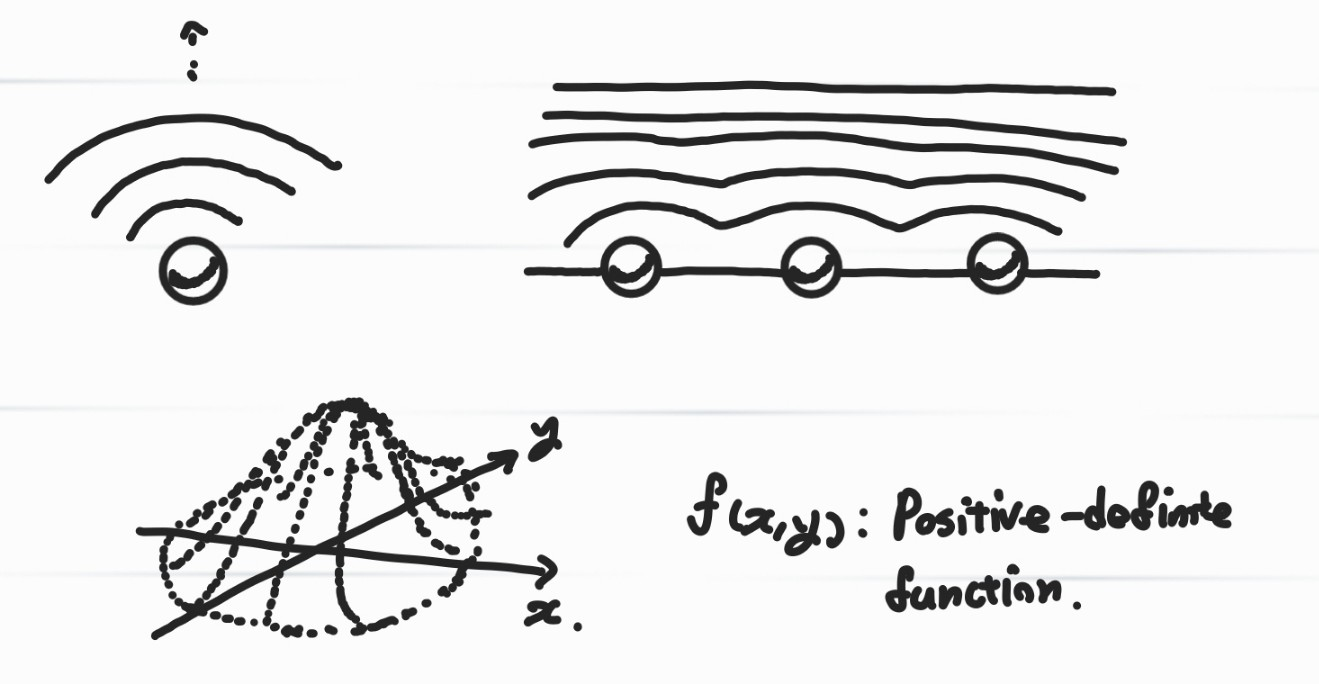
\includegraphics[width=0.8\textwidth]{media/source_distribution.jpg}
        \captionof{figure}{Source optimization problem.}
    \end{center}
    % Matrix -imshow, 
    %

    \begin{itemize}
        \item Radiation on the given surface = $\mathbf{r}$
        \item Propagation matrix = $K$
        \item Source distribution: $\mathbf{x}$, binary vector
    \end{itemize}
    
    \begin{equation*}
        K\mathbf{x} = \mathbf{r}
    \end{equation*}
    
    We want to obtain a flat radiation to some area far from the source plane, so let us apply difference matrix to both term. 
    If flatness is achieved, then the right term would be zero.

    The radiation function is $f(x) = (1+ x^2)^{-1}$
    This problem could be converted to a quadratic optimization problem by next equation.
    \begin{equation}
        \min \mathbf{x}^T A \mathbf{x}
    \end{equation}
    where, $A = Q^TQ, Q = D K$.
    The optimal solution is 
    \begin{equation*}
        \mathbf{x}_{opt} = \begin{bmatrix}
            1& 1& 0 & 1 & 0 & 1& 1&
        \end{bmatrix}
    \end{equation*}
    Since, $A$ is Hermit matrix so that we can interpret it as givein Hamiltonian.
\end{example}

You can refer a Pennylane and D-Wave implementation code of the result written by the author\cite{Kim_adiabatic_implementation}.

\subsection{Example QUBO}

Quadratic unconstrained binary optimization problem.
It is widely tried in adiabatic computation and 
in gate-model computation VQE(Variational Quantum Eigensolver) method is 
dominant however, in this chapter we will solve the 
QUBO problem on gate model computer mimicing the adiabatic process.




\begin{equation}
    D K \mathbf{x} = D \mathbf{r} = 0
\end{equation}





\subsection{Ising model}

\section{Pennylane implmentation}

\subsection{Graph partitioning problem}



